
\documentclass[a4paper,11pt]{article}
\usepackage{blindtext}
\usepackage{titlesec}
\usepackage{lmodern}
\usepackage{abstract}
\usepackage{pdfpages} %to include pdfs in the file
\usepackage{booktabs,threeparttable} %for comments to tables
\let\tnote\relax % https://tex.stackexchange.com/questions/51131/using-ctable-package-with-apa6-class?utm_medium=organic&utm_source=google_rich_qa&utm_campaign=google_rich_qa
\usepackage{geometry}
\hyphenpenalty=6000
%minimizes hyphenation
\usepackage{amsfonts} %for nice mathematical expressions
%\usepackage{acronym}
%package for table of acronyms
%\usepackage[colorinlistoftodos]{todonotes}
\usepackage{chngcntr}
%\counterwithout{figure}{section}
\usepackage{lscape}
\usepackage{longtable}
%package for tables of more than 1 page
\usepackage{tabularx}
\usepackage{array}
%packages for fixing rows of tables and centerin their content
\usepackage{rotating}
%for turning text in tables
\usepackage{verbatim}
\usepackage{setspace}
\onehalfspacing
%sets 1.5 times spaces between rows
%alternative: doublespacing
\usepackage[T1]{fontenc}
%\usepackage[latin1]{inputenc}
%\usepackage[american]{babel}
%\usepackage{csquotes}
\usepackage{floatrow} %for having 2 graphs side by side
\usepackage{textcomp} % https://tex.stackexchange.com/questions/194083/latex-error-command-textcurrency-unavailable-in-encoding-t1
%standard code for In- and Output of signs
%Careful: american is needed for the APA citation standard
%\bibliography{biblio}
%\usepackage[style=numeric, backend=biber]{biblatex}
%\bibliography{biblio}
%\DeclareLanguageMapping{english}{american-apa}
%\usepackage[style=apa, backend=bibtex]{biblatex}
\usepackage[longnamesfirst,authoryear,sort,comma]{natbib}
\bibliographystyle{ecta}

\usepackage{graphicx}
\usepackage[permil]{overpic}
%Packages for graphics: graphicx for inserting the graphic and overpic to caption it
\usepackage{multirow}
%\usepackage{booktabs}
%Packages for tables: multirow for command \multirow, booktabs for refinements
\usepackage{amsmath, amsthm, amssymb} %Package for formulas, theorems etc.
\newtheorem{prop}{Proposition} % define prop to make propositions. http://tex.stackexchange.com/questions/125981/proposition-command-doesnt-work
  \numberwithin{equation}{section} %for equation numbering according to section
% \usepackage{accents} % for underbar
\usepackage{savefnmark}
%Package for saving footnotes and re-using them
\usepackage{paralist}
%Package for special lists
% To include two graphs in the same line
\usepackage{caption} % https://tex.stackexchange.com/questions/37581/latex-figures-side-by-side
\usepackage{subcaption}
% For footnote in title
% https://tex.stackexchange.com/questions/392232/footnote-on-title-page-in-article/392234#392234
\usepackage[affil-it]{authblk}
\usepackage{blindtext}
\usepackage[english]{babel}
\usepackage[utf8]{inputenc}
\usepackage{tcolorbox}
\usepackage{import}
%Package for active citation and links within pdf
\usepackage[raiselinks, pdfborder={0 0 0}, bookmarksopen=true, bookmarksnumbered]{hyperref}
\newcommand{\commentfigure}{\scriptsize \textit{Notes: }}

%CAREFUL: needs to be at the end!
\hypersetup{hidelinks,
urlcolor=blue
}

\begin{document}

\title{Coreferences in REL
}



\author{\textsc{Flavio Hafner}
}
\affil{Netherlands eScience Center}

\date{\today}


\clearpage
\maketitle
% ABSTRACT NEEDS WORK

\tableofcontents



\section{Introduction}

REL is a software for entity linking. Entity linking consists of three steps: mention detection, candidate selection, and entity linking. Before entity linking, the current version of REL looks for coreferences in the detected mentions. Consider the example text: "This sentence is about Jimi Hendrix. The music of Hendrix is popular." Here, the second mention "Hendrix" refers to the entity "Jimi Hendrix" in the preceding sentence. Now, for each mention $m_i$, REL checks whether there is another mention $m_j$ that contains mention $m_i$ as a separate word. Denote the set of mentions $m_j$ that $m_i$ refers to by $R_i$.
If $R_i$ is a singleton, REL replaces the original candidate entities of $m_i$ with the candidate entities of $m_j$.
If $R_i$ contains multiple elements, the union of the unique candidate entities for all mentions  $m_j \in R_i$ are assigned as candidate entities for $m_i$. Moreover, for any candidate entity that appears in more than one mention $m_j \in R_i$, their $p(e|m)$ scores are aggregated for the mention $m_i$.

Coreference search can make entity disambiguation more accurate if the original candidates for mention $m_i$ are more noisy than the selected candidates for $m_j$. 
But coreference search also slows down REL for large data sets because it has quadratic time complexity.

I extend REL so that the user can choose from three options on how to deal with coreferences. The first option is "all" which corresponds to the current default of comparing all mentions with all other mentions. The second option is "off" that does not look for coreferences at all. It should be the most efficient. The third option is "lsh" that first applies locality-sensitive hashing (LSH) to all mentions, and then only searches for coreferences among mentions that are clustered together by LSH. If LSH is efficiently implemented, it could strike a balance between efficiency and effectiveness for datasets with many mentions. 

I assess the effectiveness of the three options on the AIDA data, and the efficiency on an extract from msmarco. Lacking a ground truth, I also try to check the effectiveness on these data by checking the fraction of mentions that are different between the two approaches. 

In what follows, I define coreferring mentions as mentions like the mention ``Hendrix'' above, and non-coreferring mentions as all other mentions.

The calculations are run on the CPUs of a DAS6 cluster, using Flair and the Wikipedia dump from 2019 for mention detection. I set the limit number of documents from AIDA to 500, which processes all documents. 
For the moment, I hard-code the settings for LSH in REL. The precision-recall tradeoff in LSH means that a higher recall for LSH results in a longer running time of coreference search because, for each mention, \verb|with_coref| checks more mentions. 
The current settings are set to maximize the F-score for LSH on the coreferring mentions in AIDA.



\section{Results}

\subsection{Performance on AIDA data}

Table~\ref{tab:performance_aida_full} shows precision, recall and F1 scores on the AIDA data sets (all documents) with the three options.
The three options do barely differ. The timing results show that ``lsh'' is the slowest option, and this is because setting up LSH has some overhead that dominates the value of reduced coreference search after clustering.

To compare to Erik's results (table 1 in his document), I ran REL also only with 50 documents. The effectiveness results are very similar to his results. The efficiency results, however, differ---in Erik's case, ED takes more than twice as long than in my case. I am not sure why this is.

\begin{table}
 \begin{tabular}{c c c c c c c c c c}
\hline
 coref option & \multicolumn{3}{c}{Mention detection}  & \multicolumn{4}{c}{Entity linking}  \\
    \cmidrule(lr){2-4} \cmidrule(lr){5-8}
        & Precision & Recall & F1  & Time & Precision & Recall & F1 \\
 \hline 
 ``all'' & 97.9\% & 62.9\% & 76.6\% &  11.94 sec. & 62.1\% & 39.9\% & 48.6\% \\  
 ``lsh'' & 97.9\% & 62.9\% & 76.6\% &  12.33 sec. & 62.1\% & 39.9\% & 48.6\% \\
 ``off'' & 97.9\% & 62.9\% & 76.6\% &  10.75 sec.  & 62.1\% & 39.9\% & 48.6\% \\ 
\hline 
\end{tabular}
\caption{Performance on AIDA data---all mentions. Setup: processing all documents in AIDA data set with wikipedia 2019.}
\label{tab:performance_aida_full}
\end{table}


Because only a minority of the mentions in the AIDA data are coreferences, I now check the performance for coreferring mentions only. To do this, I classify the gold mentions by whether they are coreferences or not using the same method as in REL, and then compare precision, recall and F1 scores only on these mentions. The results are in table~\ref{tab:performance_aida_corefs}. 

First, using option ``all'' , we can compare the results from the restricted sample with the results from the full sample of mentions. We see that recall for mention detection for coreferring mentions is much worse than for non-coreferring mentions---less than 40 percent of coreferring gold mentions are detected, while 60 percent of all gold mentions are detected. 
This could be (1) because coreferences are harder to detect, or (2) because some detected mentions are not labelled as coreferences because the mention they are referring to is not detected. I think case (1) is more likely.
The tables also indicate that in the ED step, REL has a higher precision but a lower recall for coreferring mentions than non-coreferring mentions. 

Second, comparing effectiveness of ED for the three options, we see that ``lsh'' performs better than ``off'' but worse than ``all''. 


\begin{table}
 \begin{tabular}{c c c c c c c c c c}
\hline
 coref option & \multicolumn{3}{c}{Mention detection}  & \multicolumn{4}{c}{Entity linking}  \\
    \cmidrule(lr){2-4} \cmidrule(lr){5-8}
     & Precision & Recall & F1 & Time & Precision & Recall & F1 \\
 \hline 
 ``all'' & 90.7\% & 36.7\% & 52.3\% & --- & 78.8\% & 31.9\% & 45.4\% \\  
 ``lsh'' & 90.7\% & 36.7\% & 52.3\% & --- & 78.8\% & 31.9\% & 45.4\% \\
 ``off'' & 90.7\% & 36.9\% & 52.5\% & --- & 76.8\% & 31.3\% & 44.4\% \\ 
\hline 
\end{tabular}
\caption{Performance on AIDA data---coreferring mentions. Setup: processing all documents in AIDA data set with wikipedia 2019. The timing is not reported because the results are taken from the same run as the results in table~\ref{tab:performance_aida_full}.}
\label{tab:performance_aida_corefs}
\end{table}


\subsection{Performance on msmarco data}

\subsubsection{Effectiveness}

To get an idea of recall and precision despite not having a ground truth, I compare the linked entities for mentions with options ``off'' and ``lsh'' to the linked entities with option ``all''. 
During the run with ``all'' I also label mentions as whether they are coreferring or not. This allows me to focus on these mentions in the following analysis.


\paragraph{Approximating recall}
One can compare whether some mentions that are linked to an entity with ``all'' are not linked with the other options. 
The option ``off'' finds 0.8 percent fewer coreferring mentions than ``all''. ``lsh'' finds 0.1 percent fewer mentiosn than ``all''. 
This suggests that recall is very similar for all options, and that ``lsh'' is slightly better than ``off''. 


\paragraph{Approximating precision}
Now I focus on the mentions that are linked. I start by comparing the fraction of mentions that have the same predicted entity by aggregating across all documents. Table~\ref{tab:performance_msmarco_avg} shows the results.
Nearly all mentions that are not coreferring have the same linked entity. 
But among coreferring mentions, when using ``off'' only 38 percent of mentions have the same linked entity. 
This implies a substantial variability in the precision of the linked entities for coreferring mentions. But the lack of ground truth prevents from drawing conclusions about whether ``off'' is better than ``all''. 
When using ``lsh'', 80 percent of mentions have the same linked entity.

\begin{table}
 \begin{tabular}{c c c c c c c}
 \hline
    & \multicolumn{3}{c}{``off''} & \multicolumn{3}{c}{``lsh''} \\
    \cmidrule(lr){2-4} \cmidrule(lr){5-7}
   coreferring mention & count & mean & std & count & mean & std \\
 \hline 
 no & 1440719 & 0.99 & 0.08 & 1440719 &	0.999 &	0.05 \\  
 yes & 97220 & 0.38 & 0.49 & 97220 & 0.80   &	0.40	 \\ 
\hline 
\end{tabular}
\caption{Fraction of mentions for options ``off'' and ``lsh'' with the same linked entity as in option ``all''.}
\label{tab:performance_msmarco_avg}
\end{table}

To check whether there is a correlation between document length and precision, I calculate the overlap by document and use the option ``all'' as a benchmark. Specifically, for the options ``off'' and ``lsh'', I calculate the fraction of mentions that are linked to the same entity like when using the option ``all''.

Starting with the opton ``off'', figure~\ref{fig:msmarco_overlap_off} plots the overlap separately for all mentions, coreferring mentions, and non-coreferring mentions. The x-axis is the total number of linked mentions in a document.
All panels show the data for documents with at least five coreferring mentions.

The figure shows considerable variation in the overlap of the predicted entities overall, stemming from variation in the overlap for the coreferring mentions. The data do not allow to draw conclusions about whether there is a relation between the number of linked mentions in the document and the overlap in the predicted entities for coreferring mentions.

\begin{figure}[H]
  \centering
  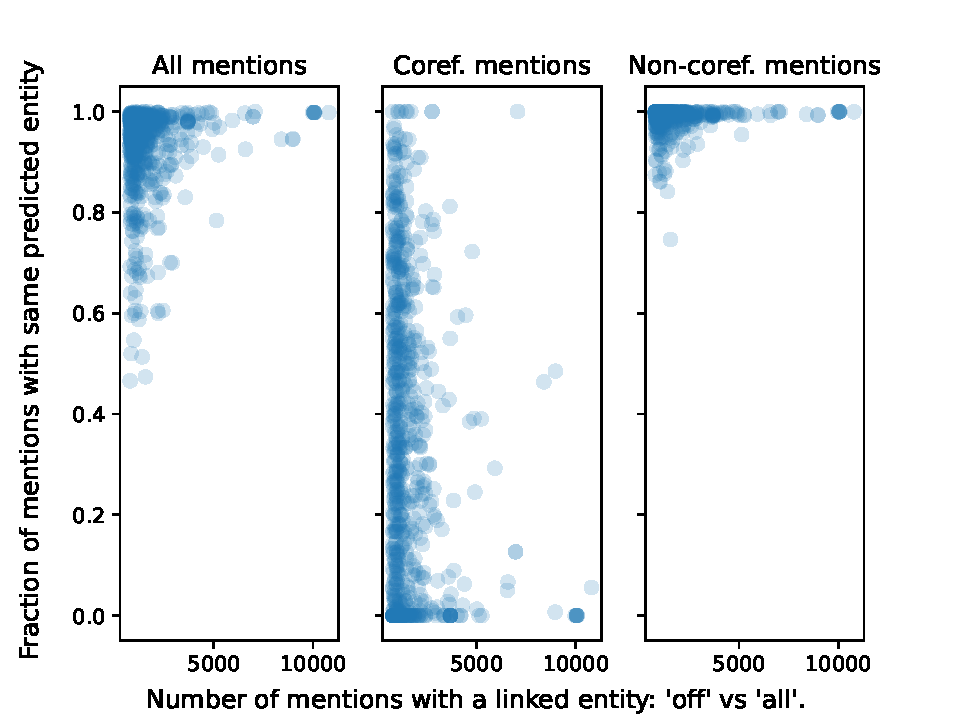
\includegraphics[width = 0.8\textwidth]{../figs/msmarco_overlap_off.pdf}
  \caption{Overlap in predicted entities, by mention type. The panels refer to all mentions, coreferring mentions and non-coreferring mentions; each mention is either coreferring or not. The unit of observation is the document. }
  \label{fig:msmarco_overlap_off}
\end{figure}

For the option ``lsh'', figure~\ref{fig:msmarco_overlap_lsh} compares ``lsh'' with ``all''. In line with the aggregate results from table~\ref{tab:performance_msmarco_avg}, ``lsh'' has a higher overlap for coreferring mentions, and perhaps even for non-coreferring mentions.

Overall, however, there is no obvious correlation between the number of mentions in a document and the fraction of mentions linked to the same entity, relative to the option ``all''. 

\begin{figure}[H]
  \centering
  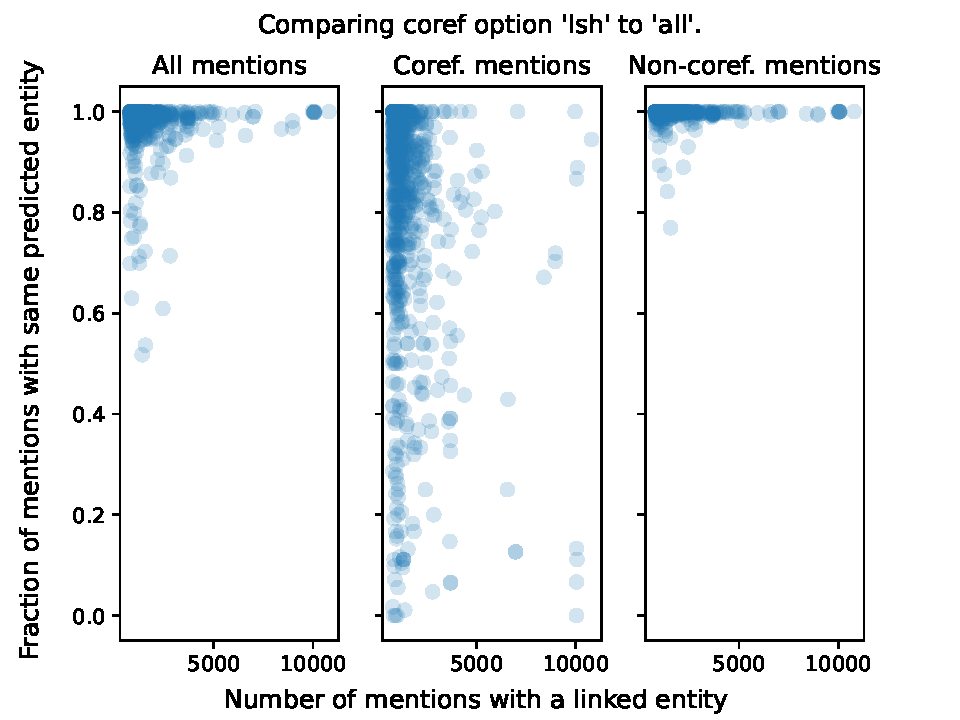
\includegraphics[width = 0.8\textwidth]{../figs/msmarco_overlap_lsh.pdf}
  \caption{Overlap in predicted entities, by mention type. The panels refer to all mentions, coreferring mentions and non-coreferring mentions; each mention is either coreferring or not. The unit of observation is the document. }
  \label{fig:msmarco_overlap_lsh}
\end{figure}


\subsubsection{Efficiency}

I now compare the running time for the options. Figure~\ref{fig:timing_msmarco} shows the running time of entity linking as a function of document size; it confirms the findings on the time complexity with the synthetic AIDA data:  the running time for ``off'' and ``all'' is not very different for documents with a few thousand mentions. 
Starting from a document size of about 6000 mentions, it appears that the option ``all'' starts to take more time for ED, while options ``lsh'' and ``off'' continue on the same trend.
These patterns are consistent with three facts: the theoretical quadratic $O(n^2)$ complexity of the option ``all'', the theoretical $O(\log{n})$ time complexity of the option ``lsh'', and the large overhead of the function \verb|predict| (see notebook for details), which  empirically seems to dominate the running time for documents with 6000 mentions or less.

\begin{figure}[H]
  \centering
  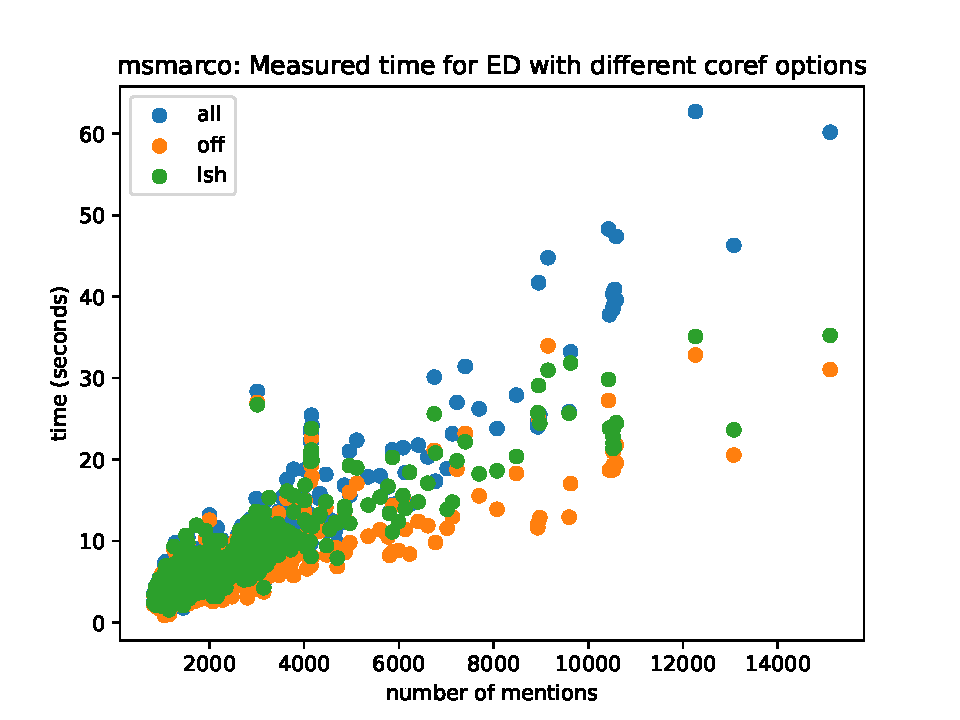
\includegraphics[width = 0.8\textwidth]{../figs/timing_msmarco.pdf}
  \caption{Time complexity on msmarco data for options ``all'', ``lsh'' and ``off''. The unit of observation is the document.}
  \label{fig:timing_msmarco}
\end{figure}



%\section{Tuning the LSH parameters}

%The LSH algorithm takes three parameters as inputs that impact the precision and recall of the clustering, which in turn impact recall and running time of the coreference search in ED.
%As of now, these parameters are hard-coded in my development branch of REL. They are chosen heuristically so that they maximize the F1-score among a set of alternative parameter values, but perhaps one can explore more rigorous ways to choose them. The ideal solution would be that they are chosen dynamically, depending on the properties of the data input. I have seen some papers that discuss this, but do not know anything about it. 



\section{Conclusion}

\subsection{Summary}
\begin{enumerate}
 \item For small input data (up to around 2000 mentions), the coreference search is inconsequential for running time. Effectiveness is highest when using option ``all'', and for coreferring mentions ``lsh'' performs equally well on the AIDA test data.
 \item For large input data, efficiency is a problem when doing a full coreference search. Particularly for documents with many coreferring mentions the choice of the option could matter, depending on how strongly coreference search impacts effectiveness in the ED step. 
 \item The results for effectiveness of ED for coreferring mentions perhaps suggest that recall is similar for either ``off'' or ``all''. But the results for precision are not clear-cut. The results from AIDA show similar precision for either option, but the results from msmarco suggest a possibly large impact on precision between options ``off'' and ``all''. 
 The option ``lsh'' is similarly effective as ``all'' but less efficient for the AIDA data; for the msmarco its predictions are much more similar to the option ``all'' than the prediction from option ``off'' are. 
 \item ``lsh'' may also speed up ED for documents with 10k mentions or more, even though there is only one such document in the msmarco data set. For smaller documents, the overhead from ``lsh'' is too large to make a difference on efficiency.  
 %I am nearing the limit for optimizations with my from-scratch solution; external alternatives such as faiss (\href{https://github.com/facebookresearch/faiss}{\underline{link}}) may be faster. 
 %\item For large input data, LSH could be a solution, but precisely in this case a time- and memory-efficient solution is key. Implementing a time-efficient LSH from scratch could take some time. There are external alternatives such as faiss (\href{https://github.com/facebookresearch/faiss}{\underline{link}}).
 \item An important reason for low recall for coreferring mentions is the mention detection, not the disambiguation, but these mentions are a small part of the total number of mentions in the AIDA data. And some of this may be resolved with the update for MD from Erik (which I have not yet integrated in my version of REL).
\end{enumerate}

\subsection{Implications}

\begin{enumerate}
 \item The coreference search option ``all'' limits the scalability of REL for documents with 6000 mentions or more.
 \item If the current implementation of coreference search is integrated in the main branch of REL, one can consider an automatic switch to either of the types of coreference search when the number of mentions is large enough, and raise a respective notification to the user. 
\end{enumerate}





%note: the current approach does not solve the quadratic time problem because the one-hot-encoding still loops through all mentions 
%is there an alternative? but in principle the algorithm does have a lower running time, so there should be a way to solve this. the first thing to do is to remove the overhead from the scipy matrix operations. 

\end{document}
